\section{Progettazione concettuale}
\subsection{Analisi dei requisiti}
% \raggedright
La base dati si deve occupare della gestione del personale di un'azienda:

la figura centrale di tutto lo schema è l'impiegato.\sskip
La prima classificazione di un generico impiegato viene fatta tra:
\begin{itemize}
	\item impiegato assunto regolarmente
	\item impiegato assunto esclusivamente per lavorare ad un progetto
\end{itemize}\medskip
Gli impiegati assunti regolarmente, vengono assunti con un determinato ruolo e stipendio, inoltre hanno diverse specializzazioni in base sia al merito sia agli anni trascorsi all'interno dell'azienda.

Dal momento in cui viene assunto, l'impiegato diventa automaticamente un junior. Trascorsi 3 anni diventa middle, trascorsi altri 4 diventa senior.
Inoltre, qualunque siano gli anni trascorsi all'interno dell'azienda, può essere promosso e diventare manager.\sskip
Si tiene traccia di tutti gli scatti di carriera all'interno dell'entità \textit{career\_log} dove sono memorizzati:
\begin{itemize}
	\item ruolo precedente
	\item ruolo successivo
	\item data dello scatto
\end{itemize}\medskip
L'azienda è divisa in varie sedi dove sono presenti diversi laboratori.\sskip
% CONTROLLARE: Un impiegato può lavorare in più laboratori anche contemporaneamente
Ogni impiegato afferisce ad un unico laboratorio.\\
Un impiegato può aver anche lavorato in più laboratori ma in periodi diversi.\\
% -----------
Al momento dell'assunzione l'impiegato non ha ancora una collocazione ma viene stabilita successivamente.\\
Ad un impiegato senior può essere assegnata la gestione di laboratori e/o di progetti.\sskip
Ad ogni laboratorio è assegnato un manager scientifico che è un impiegato senior.\sskip
L'amministratore, a cui è affidata la gestione del database, si occupa di:
\begin{itemize}
	\item inserire gli impiegati assunti
	\item monitorare gli scatti di carriera
	\item promuovere gli impiegati meritevoli a manager
	\item creare progetti e affidare la supervisione ad un manager e la gestione ad un referente scientifico
\end{itemize}\smallskip
Per ogni progetto viene stabilita una data di inizio, una \textit{deadline} per la conclusione del progetto e dei fondi.

Inoltre, si tiene traccia dell'effettiva data in cui il progetto è terminato \textit{end\_date}; può accadere che il progetto si protragga oltre la deadline\sskip
Ad un progetto possono prendere parte massimo 3 laboratori contemporaneamente.\\
Ogni impiegato che afferisce ad un laboratorio prende parte automaticamente a tutti i progetti a cui quel laboratorio sta lavorando.

Il manager scientifico di un laboratorio decide a quali progetti partecipare e abbandonare, e richiede attrezzatura.\sskip
Le richieste vengono memorizzate nell'entità \textit{equipment\_request}.
Queste vengono valutate dal manager e dal referente scientifico del progetto a cui sono state fatte, i quali decidono, in base ai fondi del progetto, se soddisfare le richieste, con il vincolo che il costo totale delle attrezzature non può superare il 50\% dei fondi del progetto.\sskip
Quando viene acquistata dell'attrezzatura, si salva l'acquisto nell'entità \textit{purchase} che tiene traccia della data e del prezzo d'acquisto.\sskip
Ogni attrezzatura di ogni laboratorio viene memorizzata nell'entità \textit{equipment}.\\
Un laboratorio può possedere già dell'attrezzatura (acquistata precedentemente da altri progetti) e riceverne altra tramite richieste a progetti. Di conseguenza l'attrezzatura acquistata in un laboratorio, rimane anche dopo la fine del progetto.\sskip
Con il restante 50\% dei fondi, il manager e il referente scientifico di un progetto possono assumere del personale che viene pagato per lavorare esclusivamente per quel progetto, e non viene considerato come impiegato regolare.

Lo stesso impiegato può essere assunto più volte (anche per lo stesso progetto ma in date differenti), per questo motivo ognuno di questi impiegati non viene rimosso una volta terminato il contratto.
La relazione \textit{works\_on} infatti, tiene traccia di tutte le volte in cui un impiegato è stato assunto per lavorare ai progetti.


\subsection{Schema concettuale}\bigskip
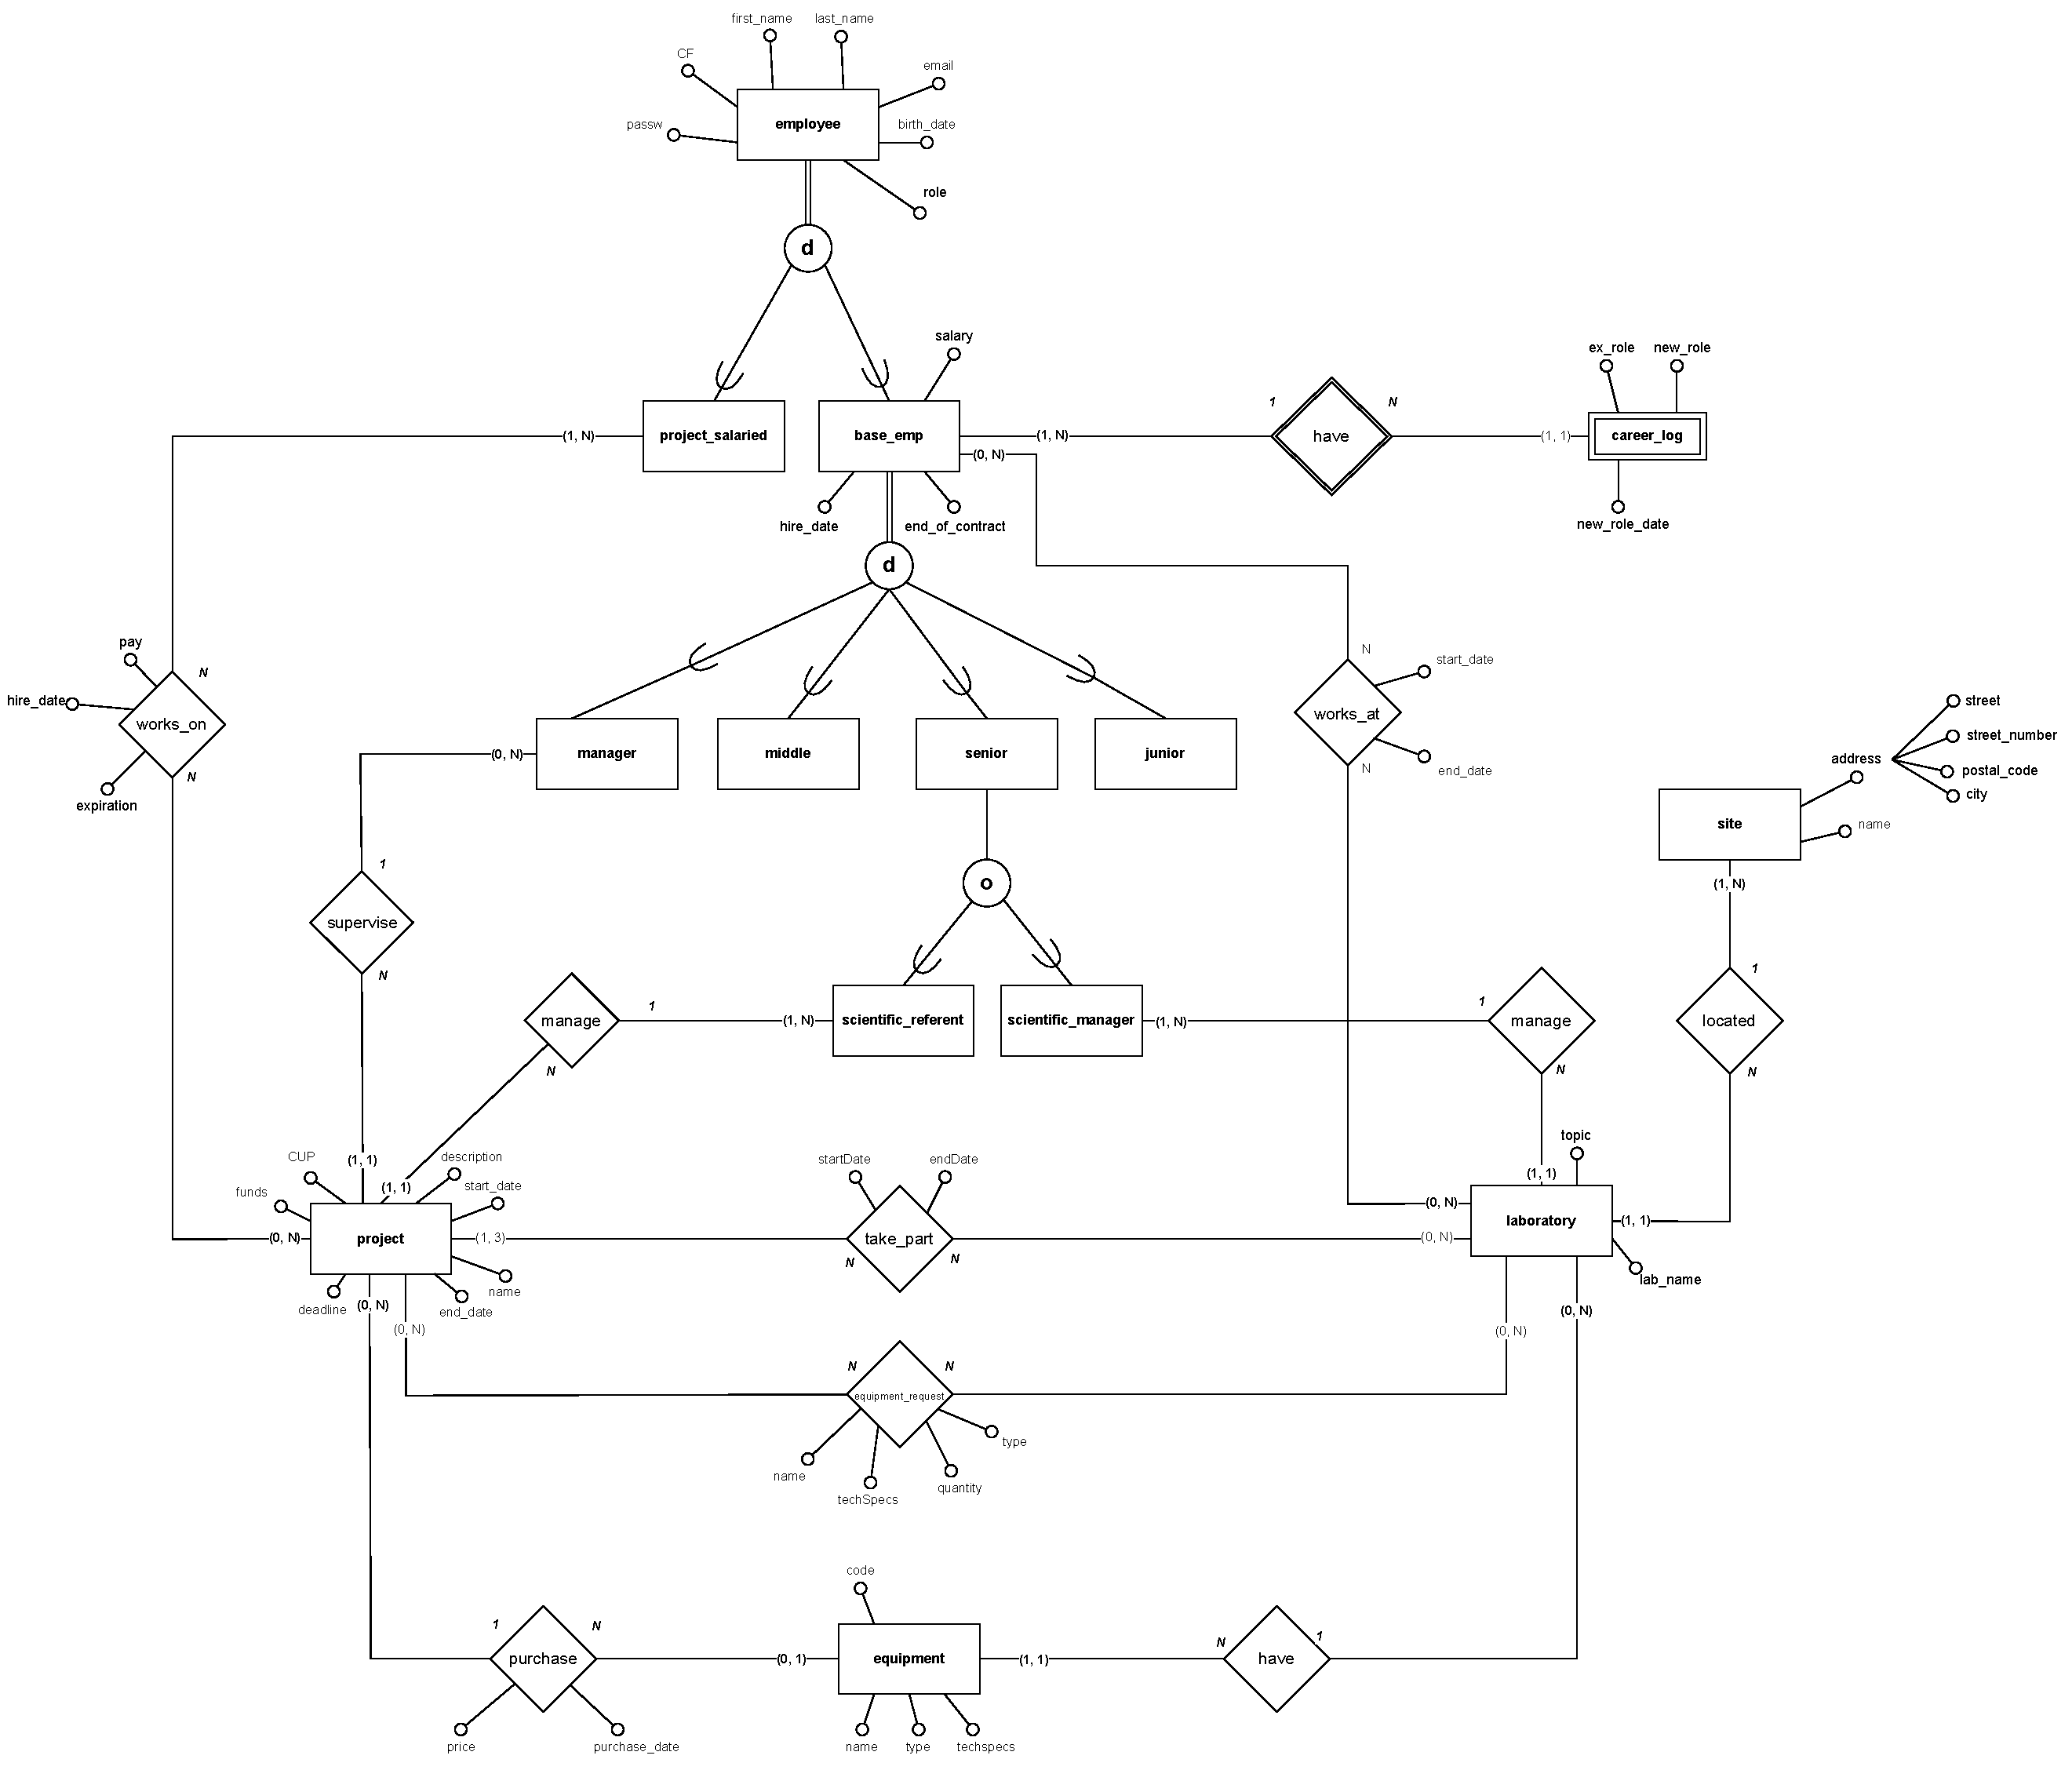
\includegraphics[width=\textwidth]{images/concettualeER.drawio.pdf}

\newpage
\subsection{Dizionario delle entità e delle associazioni}
\begin{tabular}{@{}| l | l | l |}
	\hline
	Entità & Descrizione & Attributi \\
	\hline
	col1   & col2        & col3      \\
	\hline
\end{tabular}
